\documentclass[10pt]{article}
% Packages
\usepackage{makecell} % For thicker lines
\usepackage{setspace}  % Controls line spacing
\usepackage{hhline}   % For double horizontal lines
\usepackage{colortbl}  % Add colour to LaTeX tables
\usepackage[T1]{fontenc}  % Choice of font encodings
\usepackage{tgtermes}  % Loads the TeX Gyre Termes font
\usepackage{siunitx}  % A comprehensive (SI) units package
\usepackage{tabularx, booktabs} % For advanced table layout
\usepackage{url}  % Verbatim with URL-sensitive line breaks
\usepackage{authblk}  % For author and affiliation management
\usepackage{natbib}  % A package for bibliographies and citations
\usepackage{graphicx}  % Enhances LaTeX's built-in graphics features
\usepackage{listings}  % Typeset programming code within the document
\usepackage{amssymb}  % Mathematical symbols
\usepackage[nottoc]{tocbibind}  % Adds entries to the table of contents
\usepackage{xcolor}  % Provides easy driver-independent access to colors
\usepackage{microtype}  % Improves the spacing between words and letters
\usepackage{enumitem}  % Control layout of itemize, enumerate, description
\usepackage{tocloft}  % Controls the typographic design of table of contents, etc.
\usepackage[breaklinks,linktocpage]{hyperref}  % Creates hyperlinks in your document
\usepackage[font=small,skip=7pt,labelfont=bf]{caption}  % Customising captions in floating envs

% Adjust the page margins in the bibliography
\let\oldthebibliography=\thebibliography
\let\endoldthebibliography=\endthebibliography
\renewenvironment{thebibliography}[1]{%
  \begin{oldthebibliography}{#1}%
    \raggedright%
    }{%
  \end{oldthebibliography}%
}

\setlength\bibindent{0pt}

% Optional options
% \usepackage{background} % Creates a DRAFT background image on all pages
% \backgroundsetup{contents=Preprint, opacity=0.25, color=gray} % Adds a watermark to the document
% This command changes the line spacing to double.
% ? Needed for reviews/drafts
% \doublespacing

% Custom colours
\definecolor{codegreen}{rgb}{0,0.5,0}
\definecolor{codegray}{rgb}{0.4,0.4,0.4}
\definecolor{codepurple}{rgb}{0.58,0,0.82}
\definecolor{backcolour}{rgb}{0.96,0.96,0.96}
\definecolor{lightgray}{gray}{0.8}

\lstdefinelanguage{JavaScript}{
  keywords={break, case, catch, continue, debugger, default, delete, do, else, finally, for, function, if, in, instanceof, new, return, switch, this, throw, try, typeof, var, void, while, with},
  morecomment=[l]{//},
  morecomment=[s]{/*}{*/},
  morestring=[b]',
  morestring=[b]",
  sensitive=true
}

% Listing styles
\lstdefinestyle{mystyle}{
  frame=tb,
  tabsize=2,
  captionpos=b,
  numbers=left,
  framerule=0pt,
  numbersep=5pt,
  showtabs=false,
  breaklines=true,
  keepspaces=true,
  showspaces=false,
  framextopmargin=6pt,
  framexbottommargin=6pt,
  showstringspaces=false,
  breakatwhitespace=false,
  keywordstyle=\color{purple},
  commentstyle=\color{codegreen},
  stringstyle=\color{codepurple},
  numberstyle=\tiny\color{codegray},
  basicstyle=\ttfamily\footnotesize,
  backgroundcolor=\color{backcolour}}
\lstset{style=mystyle}

% ! Custom template commands
% Add a vertical space after section numbers in ToC
\renewcommand\cftsecafterpnum{\vskip8pt}
% Changes the title of the list of listings
\renewcommand{\lstlistlistingname}{List of \lstlistingname s}
% Changes the title of the bibliography
\renewcommand{\bibname}{References}
% Changes the title of the table of contents
\renewcommand{\contentsname}{Table of Contents}
% Changes the leader between section and page numbers in ToC
\renewcommand{\cftsecleader}{\cftdotfill{\cftdotsep}}
\newcommand{\floatcaption}[2]{\caption[#1.]{#1~#2.}}

% Custom template settings
\captionsetup{justification=centering}  % All captions will be centered
\hypersetup{
  colorlinks = true,
  urlcolor = blue,
  linkcolor = blue,
  citecolor = blue,
  breaklinks = true
}
\PassOptionsToPackage{hyphens}{url}
\urlstyle{same}
\def\Urlmuskip{0mu plus 1mu}
\def\UrlBreaks{\do\/\do-}
\def\UrlBigBreaks{\do\/\do-\do:\do.}
\setlist[itemize]{noitemsep, topsep=0pt, partopsep=0pt}




\begin{document}
% Changing the initial page numbering to uppercase Roman
\pagenumbering{roman}
% Resetting the page counter to 1
\counterwithin{lstlisting}{section}
\counterwithin{figure}{section}
\counterwithin{table}{section}
% Sets the distance between the bottom and the footer
\setlength{\footskip}{65pt}

% ! ===============================
% ! Start of the title page content
% ! ===============================

\title{\textbf{Stem Cells and Epilepsy:} \\ Modelling the Brain with Organoids}
\author[ ]{Daniel Burger}
% \author[ ]{K23003985}
\affil[ ]{\textbf{King’s College London}}
\affil[ ]{\href{mailto:public@danielburger.online}{public@danielburger.online}}
\date{\textit{13. February 2024}}
\maketitle
% Resetting the page style for the first page
\thispagestyle{empty}
\doublespacing

% The sloppypar environment adjusts the spaces between words such that each line fits into the text width
\begin{sloppypar}
  \begin{abstract}
    % TODO Create the final abstract
    % NOT THE FINAL ABSTRACT: This essay examines the role of stem-cell-derived models, such as human induced pluripotent stem cells (hiPSCs) and brain organoids, in epilepsy research. Traditional in vivo and in silico models have provided foundational insights but often fail to mimic complex human brain dynamics. Stem-cell-derived models offer a closer approximation of human neurodevelopmental processes in a controlled environment, enabling detailed studies of epilepsy’s pathophysiology. The author highlights key advancements, including the modelling of developmental epilepsies and the exploration of therapeutic targets. Case studies illustrate the practical applications of these models in uncovering the mechanisms of epilepsy. The essay also touches on ethical considerations inherent to stem cell research.
  \end{abstract}

  \pagebreak
  % Changing the page numbering back to uppercase Roman
  \pagenumbering{Roman}
  % \tableofcontents
  % \pagebreak
  % \listoffigures
  % \pagebreak
  % \listoftables
  % \pagebreak
  % \addcontentsline{toc}{section}{\lstlistlistingname} % Add to the TOC
  % \lstlistoflistings
  % \pagebreak
  % Changing the page numbering back to Arabic
  \pagenumbering{arabic}

  % ! ====================================
  % ! Start of the actual document content
  % ! ====================================

  \section{Introduction}
  \label{sec:introduction}

  Epilepsy, a neurological disorder afflicting around 50 million individuals worldwide \citep{world2019epilepsy}, manifests through recurrent, unprovoked seizures as illustrated in \autoref{fig:seizure-eeg}, which can lead to symptoms such as convulsions (i.e. uncontrolled shaking), loss of consciousness, and unusual sensations or behaviours. The development of seizures in epilepsy is mainly due to a complex interaction between the excitatory and inhibitory activities of neurons in the brain. When there is an imbalance that leads to more excitation than inhibition, it can cause sudden and abnormal electrical activity in localised or entire regions of the brain \citep{robinson_propagation_1997}.

  Temporal lobe epilepsy (TLE) is the most common form \citep{epilepsy_foundation_temporal_2019}—yet it is the drug-resistant epilepsies, especially those without an identifiable epileptogenic zone, that present the most significant treatment challenges \citep{iwasaki_non-invasive_2016, guery_clinical_2021}. Current interventions, such as neuromodulation \citep{fisher_electrical_2014}, offer some hope, but their effectiveness is variable and can be marred by severe side effects, highlighting the urgent need for novel research directions.

  The impact of epilepsy extends far beyond its physiological symptoms, affecting every facet of an individual’s life. A large number of people who are diagnosed suffer from uncontrollable seizures, rendering them incapable of performing routine tasks, securing employment, or even driving—a prohibition enforced in many countries, such as e.g. Switzerland, due to safety concerns \citep{schweizerische_epilepsieliga_driving_2021}. This pervasive uncertainty cultivates a lifestyle fraught with limitations, emphasising the disease’s profound societal and personal toll.

  \begin{figure}[ht]
    \centering
    \frame{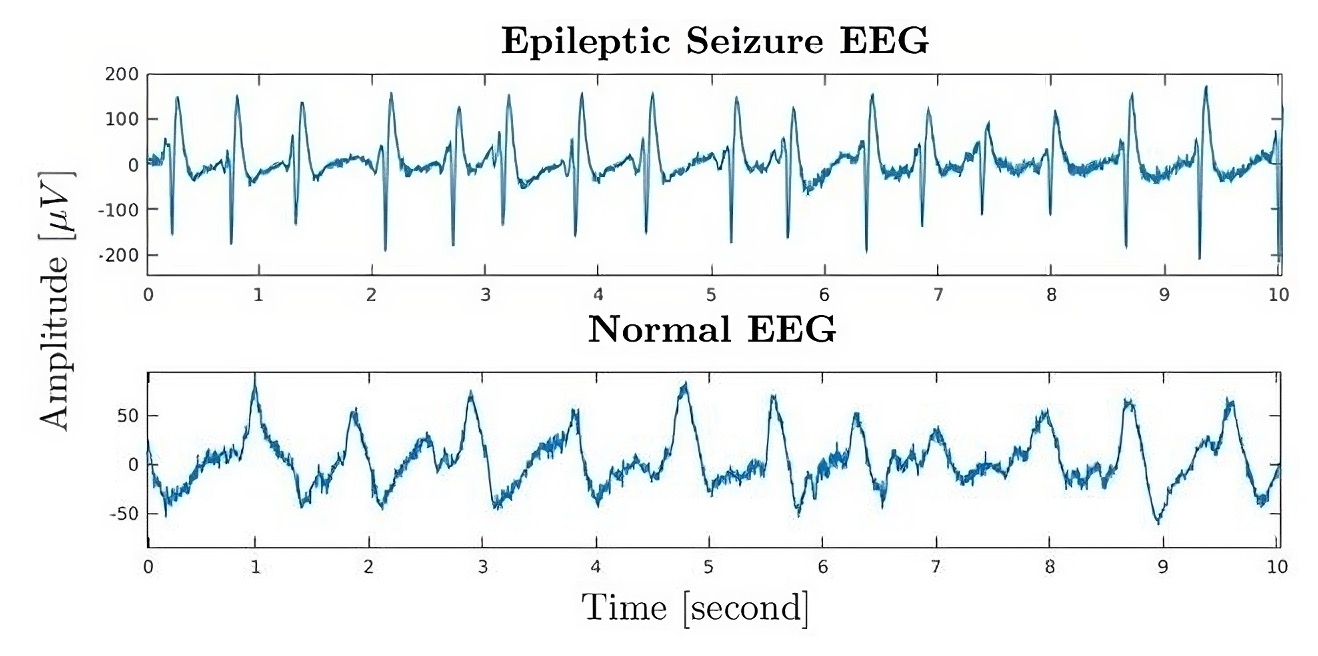
\includegraphics[width=\textwidth]{figures/seizure-eeg.jpg}}
    \caption[EEG Waveforms: Epileptic vs. Normal Brain Activity]{\textbf{EEG Waveforms: Epileptic vs. Normal Brain Activity.} Comparative display of EEG waveforms showing brain electrical activity over 10 seconds. The top graph represents EEG data during an epileptic seizure, characterised by high amplitude and frequent spikes, indicative of abnormal neuronal activity. The bottom graph illustrates a normal EEG with regular wave patterns and lower amplitude, reflecting typical brain function. The x-axis measures time in seconds, and the y-axis measures the amplitude of brain waves in microvolts (µV). Image taken from \cite{espinosa_feedforward_2020}.}
    \label{fig:seizure-eeg}
  \end{figure}

  The origins of epilepsy are diverse, encompassing genetic predispositions (genotype) and observable characteristics (phenotype), including brain injuries and infections, underscoring the complexity of its etiology.

  \subsection{Traditional Models for Epilepsy Research}
  \label{sec:traditional-models-for-epilepsy-research}

  Traditional epilepsy research models, such as in vivo animal subjects and in silico simulations, have been invaluable yet present notable limitations. Animal models, often e.g. employing rodents \citep{wang_animal_2022}, provide insights but may not fully translate to human epilepsy due to differences in brain structure and function \citep{kandratavicius_animal_2014}. Similarly, in silico models, like those developed by the Blue Brain Project \citep{markram_blue_2006}, offer detailed simulations of neural networks but are limited by current computational capabilities and understanding of the brain \citep{mirza_integrative_2016}.

  Stem-cell-derived models, mainly from human induced pluripotent stem cells (hiPSCs), emerge as a promising solution, offering a more accurate and ethical approach to studying epilepsy. Unlike animal models, which face translational hurdles due to species-specific differences in brain architecture and function, hiPSCs can be derived from human cells, ensuring a closer representation of human pathophysiology. Furthermore, the use of hiPSCs sidesteps the ethical quandaries associated with embryonic stem cell research, as they can be obtained from adult cells (e.g. skin cells) without harm to the donor, thereby aligning with ethical standards for human research \citep{takahashi_induction_2006}. These models circumvent traditional methods’ limitations by providing a renewable source of human neural tissue and enabling the exploration of epilepsy’s neurodevelopmental and pathophysiological aspects in a patient-specific context while allowing precise analysis and imaging of the tissues in a highly controlled environment.

  \subsection{Current State of the Art}
  \label{sec:current-state-of-the-art}

  The advances in stem cell technology have given rise to another groundbreaking approach: cultivating three-dimensional brain organoids derived from hiPSCs. Compared to the previously mentioned approaches where neuronal cells were usually cultivated in a two-dimensional manner (sometimes called dish brains), researchers can now generate brain organoids that mimic the brain’s complex architectures in terms of tissue structures and the arrangement of cellular types, cell-to-cell interactions, and synaptic connectivity, surpassing two-dimensional dish brains that fall short in replicating the physiological interactions, regional specificity, and microenvironment gradients observed in vivo \citep{clevers_modeling_2016, wang_modeling_2018}.

  Another benefit of cultivating brain organoids is that it allows researchers to grow or 3D-print neural tissue, e.g. around electrically conductive matrices or electrodes \citep{yao_3d_2023}, engaging with and measuring the organoids in ways reminiscent of living brains. Additionally, combining multiple brain organoids as an assembloid offers a sophisticated method to study the interactions between different brain regions \citep{sloan_generation_2018} as they, e.g. facilitate the inter-regional synaptic connections critical for higher-order brain functions, often disrupted in epilepsy.

  \section{Discussion}
  \label{sec:discussion}

  % TODO: Write a short intro to the discussion section (in the public essay)

  \subsection{Stem-Cell-Derived Models for Epilepsy}
  \label{sec:stem-cell-derived-models-for-epilepsy}

  One of the most compelling aspects of hiPSC technology is its ability to model genetic forms of epilepsy. By deriving iPSCs from patients with known genetic mutations, researchers can observe the direct effects of these mutations on neuronal development, function, and network formation. This approach has been instrumental in elucidating the pathophysiological mechanisms underlying syndromes such as, e.g. Dravet Syndrome and Tuberous Sclerosis Complex, where specific gene mutations lead to distinct epileptic phenotypes \citep{jiao_modeling_2013, nadadhur_neuron-glia_2019}.

  \begin{figure}[!ht]
    \centering
    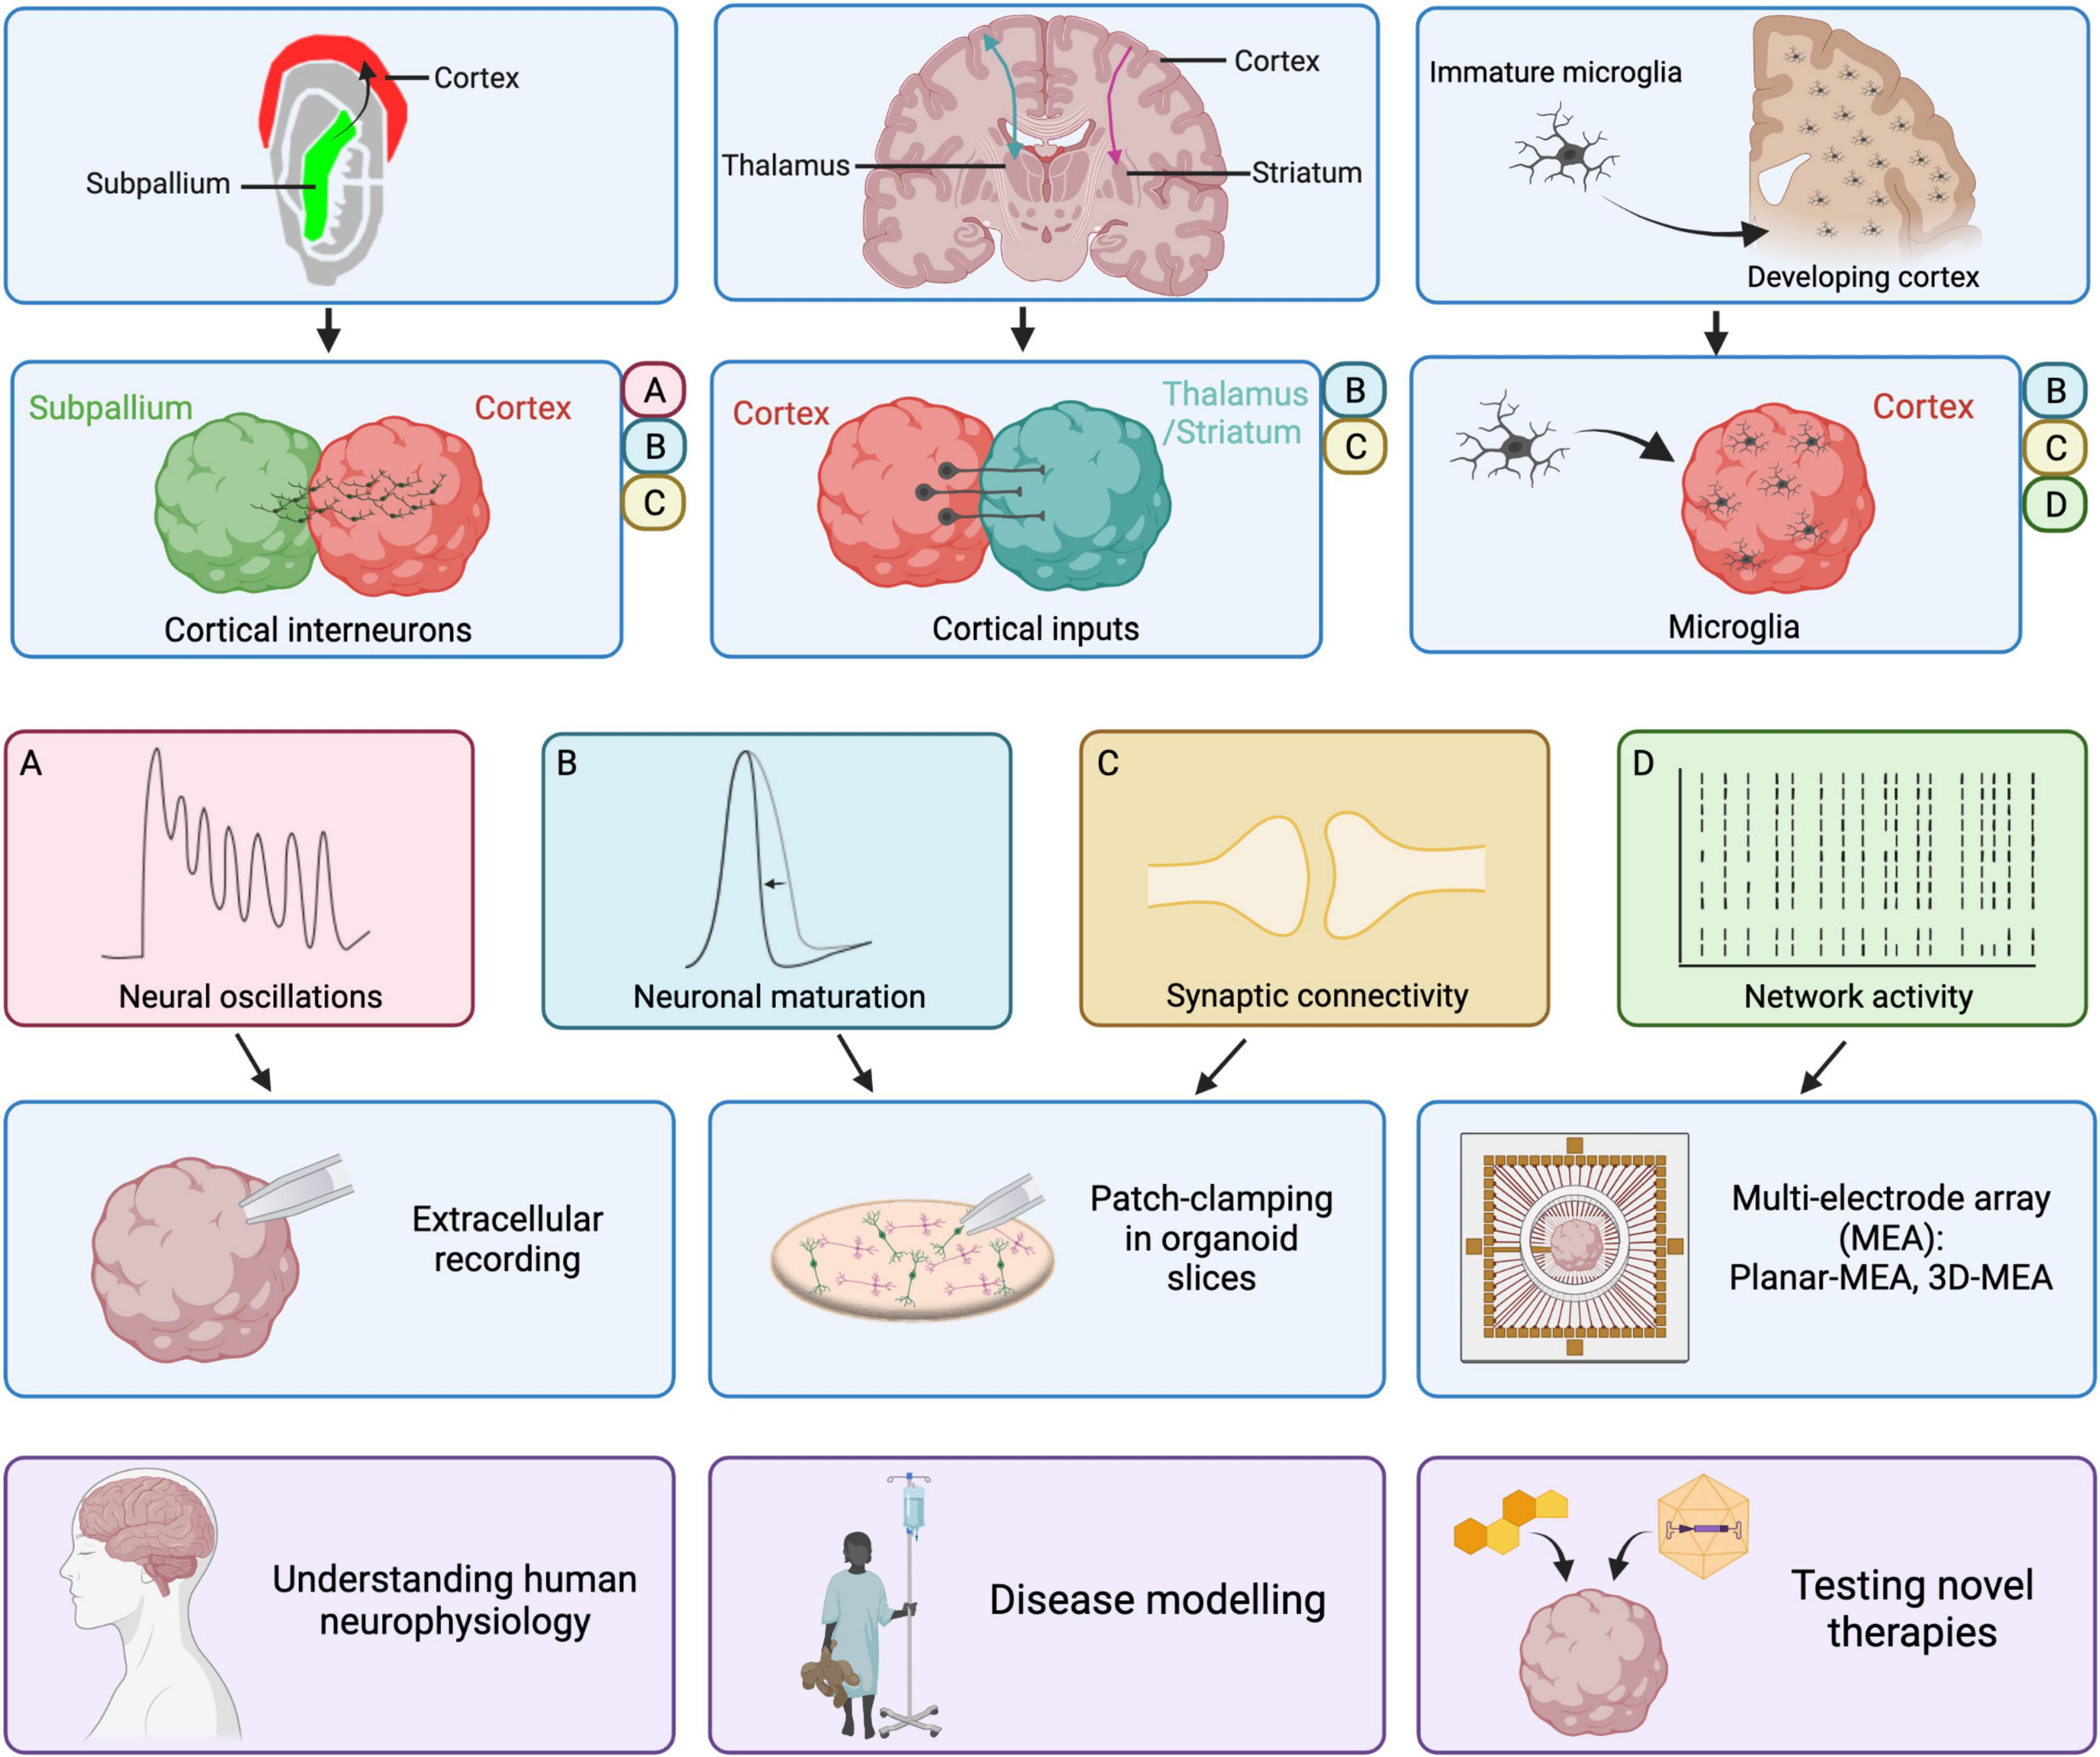
\includegraphics[width=\textwidth]{figures/organoid-advancements.jpg}
    \caption[Advancements in Cortical Organoid Models]{\textbf{Advancements in Cortical Organoid Models and Their Electrophysiological Characterisation.} This figure illustrates the enhancements in cortical organoid models, emphasising the integration of cortico-subpallial, cortico-thalamic, and cortico-striatal assembloids, as well as the addition of microglia. A) The emergence of neural oscillations, B) Neuronal maturation with a shorter action potential (AP) half-width, C) Increased synaptic connectivity, and D) Elevated network activity are depicted through electrophysiological recordings. These advancements provide a more accurate approximation of human neurophysiology and present new possibilities for disease modelling and testing novel epilepsy therapies. Image taken from \cite{zourray_electrophysiological_2022}.}
    \label{fig:organoid-advancements}
  \end{figure}

  Despite these advances, stem-cell-derived models of epilepsy face several challenges. The differentiation of iPSCs into fully mature, functional neurons and glial cells that accurately represent the diversity and complexity of the human brain remains a daunting task. This is particularly pertinent in modelling age-related epilepsies, where the disease phenotype may only manifest or worsen over time. As mentioned earlier, techniques such as 3D brain organoids or assembloids, depicted in \autoref{fig:organoid-advancements}, have emerged as a promising solution to mimic the brain’s architecture and cellular heterogeneity more closely, though they are not without their own set of limitations, including the lack of vascularisation and an immune system \citep{lancaster_cerebral_2013, di_lullo_use_2017}.

  Recent studies, such as those by \citeauthor{thodeson_neural_2017} \citeyearpar{thodeson_neural_2017}, underscore the potential of neural stem cells in epilepsy research. These investigations reveal that iPSC models can uncover novel insights into diseases with epileptic phenotypes despite challenges such as variable expression profiles and differentiation potential among iPSC lines. For example, iPSC models of Rett syndrome, a rare genetic disorder that leads to severe cognitive and physical impairments such as seizures, have illuminated critical aspects of epileptogenesis by demonstrating decreases in neuronal soma size, neurite outgrowth, and synapse formation compared to controls, thereby highlighting the intricate interplay between neuronal and astrocytic contributions to the disease \citep{marchetto_model_2010}.

  The evaluation of stem-cell-derived models’ effectiveness and limitations, as discussed by \citeauthor{kandemir_investigation_2022} \citeyearpar{kandemir_investigation_2022}, points to the nuanced relationship between neurogenesis and epilepsy. However, the specificity of neurogenesis markers and the role of mature astrocytes in epilepsy remain areas of ongoing research, emphasising the need for continued innovation and refinement in stem-cell-derived epilepsy models \citep{jessberger_epilepsy_2015}.

  \subsection{Case Studies and Practical Applications}
  \label{sec:case-studies-and-practical-applications}

  Building on the foundational concepts discussed earlier, we now shift our focus to two pivotal case studies and practical examples. These instances illustrate the real-world application of stem-cell-derived models in epilepsy research.

  \vspace{0.5cm} % Add empty line

  \begin{itemize}[leftmargin=*]
    \item \textbf{Samarasinghe et al. (2021)} looked into the complex neural dynamics of brain organoids, uncovering significant epileptiform activities within organoids modelling Rett syndrome. However, \citeauthor{samarasinghe_identification_2021} groundbreaking work demonstrated the presence of sophisticated physiological activities within these organoids and the potential for therapeutic intervention. Remarkably, they observed a substantial reduction in epileptiform activities upon administration of pifithrin-$\alpha$, a TP53 inhibitor, which points towards new directions in epilepsy treatment, especially for conditions exhibiting resistance to conventional therapies.

    \item \textbf{Steinberg et al. (2020)} undertook an ambitious project to model epileptic encephalopathies using a combination of CRISPR-engineered human embryonic stem cells and patient-derived iPSCs, focusing on the devastating WOREE syndrome, a rare neurodevelopmental disorder characterised by drug-resistant epilepsy and global developmental delay. Their meticulous approach unveiled significant cellular and molecular CNS abnormalities, including alterations in GABAergic markers, which suggest a disruption in the development of normal and balanced neuronal networks. This work not only underscores the intricate pathophysiology of epileptic encephalopathies but also provides a proof-of-concept for potential therapeutic interventions, such as the modulation of GABAergic responses, which are crucial in the dynamics of developmental epilepsies.
  \end{itemize}

  \subsection{Other Approaches and Advancements}
  \label{sec:other-approaches-and-advancements}

  It should have become evident so far that stem cell technology shows promise in epilepsy research, especially what is to come to tackle this disease. Among the most promising developments is the transplantation of hiPSC-derived brain organoids into living beings, a technique that has shown significant potential in increasing inhibition in epileptic brain areas. \citeauthor{hunt_interneuron_2015}’s \citeyearpar{hunt_interneuron_2015} pioneering work on interneuron transplantation laid the groundwork for this approach, demonstrating the feasibility and therapeutic potential of grafting new inhibitory neurons into the epileptic brain.

  Building on this foundation, \citeauthor{neurona_neurona_2022} \citeyearpar{neurona_neurona_2022} has made significant strides with its lead cell therapy candidate, NRTX-1001, which is currently being evaluated in a Phase 1/2 clinical trial for people with drug-resistant mesial temporal lobe epilepsy (MTLE). The therapy involves a one-time administration of fully-differentiated neural cells, called interneurons, derived from hiPSCs and intended to provide long-term GABAergic inhibition to repair hyperexcitable neural networks. Early results from the clinical trial are promising, with significant seizure suppression and no serious adverse events reported in patients treated with NRTX-1001. These findings suggest that NRTX-1001 could represent a groundbreaking, non-destructive treatment for epilepsy, offering hope for durable seizure reduction and improved quality of life for individuals living with this debilitating condition.

  \subsection{Ethical Considerations}
  \label{sec:ethical-considerations}

  While working with stem cells, we are nonetheless confronted with many ethical considerations that demand our attention. \citeauthor{farahany_ethics_2018} \citeyearpar{farahany_ethics_2018} provide a comprehensive overview of the ethical landscape when experimenting with human brain tissue, raising critical questions about the moral implications of in vitro experimentation.

  The ethical discourse surrounding brain organoids primarily hinges on their increasing complexity and the theoretical possibility of these entities attaining a form of consciousness or subjective experiences. This prospect, albeit currently small, necessitates a careful examination of the moral status of these organoids and the protections they might warrant, akin to those provided to human or animal research subjects.

  One of the significant ethical challenges lies in the limitations of current brain organoid models, particularly their lack of a comprehensive vascular system, which restricts their growth and complexity, as mentioned in \autoref{sec:stem-cell-derived-models-for-epilepsy}. Therefore, the potential to create sentient brain organoids in laboratories emerges as a topic of ongoing debate and research, necessitating a cautious and principled approach to ensure we do not inadvertently cross ethical boundaries.

  \section{Conclusion}
  \label{sec:conclusion}

  The shift towards stem-cell-derived models, particularly in epilepsy research, marks a significant advancement over traditional methods like animal testing and in silico simulations. These models, through the use of hiPSCs and brain organoids, offer a more accurate representation of human brain physiology, propelling us toward personalised medicine. Their application has illuminated pathways for novel treatments, showcasing the potential to transform the management of epilepsy and other neurological disorders. Despite the promise, challenges persist, including technical hurdles and ethical concerns. Yet, as we navigate these complexities, the evolving landscape of stem-cell research holds the promise of groundbreaking discoveries that could redefine our approach to neurological health and treatment.

  % ! ==============================================
  % ! Start of the references and appendices content
  % ! ==============================================

  \pagebreak
  \singlespacing
  \bibliographystyle{../../templates/custom-apa}
  \bibliography{references/bibliography}

\end{sloppypar}
\end{document}
